\chapter{Migratable Applications}
\label{chap:migratableapps}

In this chapter we introduce migration-friendly applications and pinpoint
common properties among them. These speculations almost inevitably lead
us towards coming up with a certain computation model for these
applications.
The functional and performance requirements of this computation model will
ask for certain features from a hypothetical migration framework. As the
takeaway from this chapter we will infer the goals that we must pursue
in designing Slope to address those requirements.
%
%speculate api
%
%possible usecases in distributed applications
%
%design goals and important metrics
%
%where do we need to be careful

% say these are the things we need to do, lay out some requirements,
% balance tradeoffs (e.g. access at source vs how quickly do the mig,
% track allocs

\section{Migration-friendly applications}
Distributed applications refer to a large family of applications with
different functionalities and requirements. From distributed transactions
engines and RPC frameworks to data pipelines and graph processing systems,
we must identify the
applications which can naturally play along with the notion of migrating
slices of their work to their peers to achieve better load balancing.

However instead of taking a vertical slice of applications from this range
to target one of these domains, a horizontal slice possibly spanning
multiple of the domains can help us better identify the core
properties of migratable applications.

\subsection{Migratable partitions}

\autoref{fig:designgoalspluggable} shows our first sketch of a
migration-friendly application which consists of symmetric instances
running on the machines in a cluster. The application can internally
partition its units of work into partitions that can be operated or
managed either independently, or less strictly,
with well defined and infrequent cross-communication through APIs.
This partitioning scheme could be natural, like
partitioning user data data based on the user id, or it could be driven
by a pure need for load balancing, such as randomly sharding the data
in a transaction processing system.


\begin{figure}[t]
\centering

\ensurepdffromsvg{design-goals-pluggable.drawio}
\includegraphics[width=0.5\textwidth]{design-goals-pluggable.drawio}
\caption{
    The migration platform allows the already partitioned units of
    data/computation to be migrated across machines. \ANGELA{stop writing
    paragraphs in captions. Application partitions
    are the self-sufficient, independent units of work and therefore the
    migratable objects in this system.}
}
\label{fig:designgoalspluggable}
\end{figure}

An immediate gain of the application from this model is load balancing,
while retaining locality of access and in case of repeated requests to
the applications, cache locality.
Given that the application can decompose its data and processing into
partitions that are small enough, it can use the migration platform to
spread
out its load evenly across the cluster. In time-sensitive applications
if the load is dynamic,
meaning the need to rebalance the workload arises frequently,
then the migration platform must also work in real-time.

In these applications each shard or partition will likely provide the
full API of the whole system. In \autoref{fig:designgoalspluggable},
if the workload did not contain partitions 2 and 3, then the only
    difference in the transition from top to bottom would have been the
    thin API wrapper around its partition which is responsible for tasks
    such as routing the requests to the correct machine. Otherwise
    Partition 1 would look like the whole application from the outside.

Therefore apart from the run-time load balancing benefit, the
    migration platform also simplifies a part of the development of the
    application: the system designer needs to program to an
    \emph{application partition}, as opposed to programming to the
    \emph{whole system}. This separation of concern,
    by definition breaks the dependency between how
    any shard handles a request to its API and what the rest of the
    platform does, including how request routing or replication is done
    in the application. Note that the need for request routing or
    replication are not implications of the partitioned computation
    model: we had to go distributed already to meet the requirements of
    the big workloads, but in a partitioned model we can think about those
    in isolation without propagating their complications to the
    core of the application.


\begin{figure}[tp]
\centering

\ensurepdffromsvg{migration-transport.drawio}
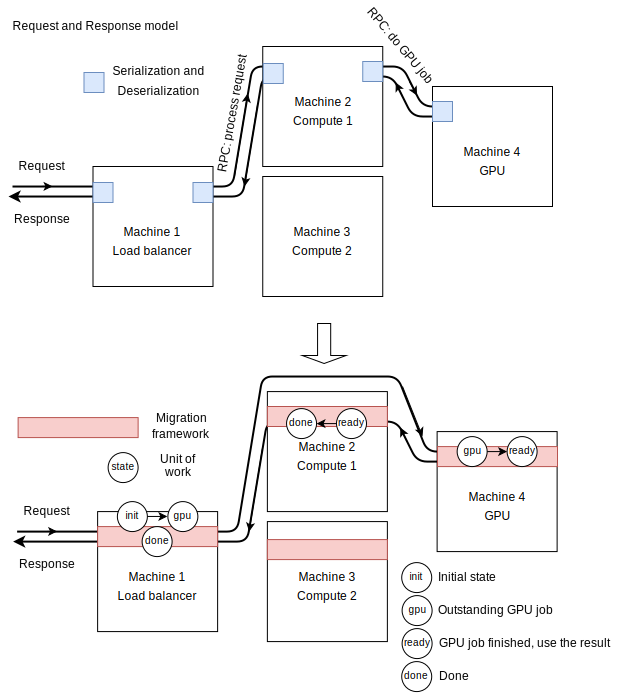
\includegraphics[width=0.8\textwidth]{migration-transport.drawio}
\caption{
    Using a migration platform as the transport in a system with
    application level routing/load balancing. The system needs to execute
    the data parallel computation portion of each task on the machine
    which has a GPU. A request/job is the
    migratable element in this scenario. Each request is independent
    from other requests. Each request is also self sufficient as its
    state identifies what action and by which machine type must be
    executed on the object. Each node executes its share of work
    on the request object based on its current state, updates the state by
    writing to the object memory, and migrates it to the next hop based
    on the state.
}
\label{fig:migrationtransport}
\end{figure}

\subsection{Migratability as a transport}
\ANGELA{Talk about the state machine directly, and focus on the positive}
With certain performance qualifications, a migration framework can act as
an intra-cluster transport. Example use cases for such a transport arise
in application level (or layer 7 in OSI terms) routers in heterogeneous
computation environments. \autoref{fig:migrationtransport} depicts
a simple example of this use case. 


From a performance point of view, this makes little difference to the
application if there is serialization involved. In fact we could have
even framed
serialization and deserialization and RPC as a migration framework. If we
could do the migration in a ``pure'' way, meaning we could ideally
eliminate the serialization and deserialization, limiting what is sent
over the wire between each pair of servers to a minimum, the applications
performance has a chance of improvement. If we were able to hand off
objects between servers in a way that is not different from calling a
function on the same server, the two servers will in essence look
``closer'' to each other both from a performance and a programmability
point of view. The former will result in improvements in run-time and
the latter will empower system designers.

The difference between this computation model and a general
request-response or RPC model is that the unit of work is a
well defined object and each step in the computation can be
efficiently modeled as doing certain computation work and then taking
the object to the next state. This will rarely resemble the computation
model of an application that is modeled as a number of completely separate
services, or how a mobile client would communicate with the application
server.

From a different angle, this model allows us to choose a tightly
coupled set of performance critical tasks in an application with
heterogeneous data or computation requirements, and model their
communication using a framework which hides low level networking details
and takes away the need to serialize or deserialize payloads.
This is an improvement in programmability. With little development
effort and no complications in the design of the application,
we can build, maintain and
extend sub-systems which can carry out tasks across multiple machines.

\subsection{Core properties of a migration framework}
\label{subsec:coreprops}

The function of a migration platform is to provide a mechanism to allow
applications to seamlessly move their data structures and their
corresponding operations across their instances.

\paragraph{Real-time performance:}
We define migration delay to be the elapsed time since the start of the
migration of an object until it is successfully migrated to its
destination. Based on the two application types that were discussed,
the most
important feature of a migration framework is its ability to keep the
migration delay small to allow migrations to happen in real-time.
However this is not particularly insightful in designing such a system.
All applications will prefer a smaller end-to-end migration delay
if all of their other metrics are left unchanged. Similarly exceedingly
    large migration delays will interfere with the performance of
    virtually all applications. Furthermore, directly measuring this
    duration and pursuing its optimization as the main performance goal
    may fail to reflect how the migration process impacts the application.
    For example some applications may prioritize responsiveness and
    would trade off
    some of their throughput during the migration process to keep their
    tail latencies low.  Therefore it makes more sense to define migration
    performance from the view point of the application based on how
    \emph{its} performance metrics degrade as a result of the migration.
    While there is value in keeping the migration delay small, we must
    prioritize maximizing the \emph{usefulness} of the application in
    the distributed setting during the migration.

\paragraph{Pluggability and Programmability:}
A fast migration mechanism comes at a cost. After all, each application
could theoretically hand craft and micro-optimize its networking protocol,
but this will complicate the design of the application by propagating
the complexities of the low level protocol into the core of the
application. This will make it difficult to maintain and improve the
application since a small change in how the application carries out its
task may break the preconditions of the custom protocol. Therefore as the
second core requirement of migration platforms, 
we will aim for zero modification to the
internals of the application and minimal addition to the API of the
units of computation. That means if
the system designer has already come up with a way to partition
data and computation into units that can be run independently on
possibly different machines, the task of integrating the migration
platform into the system to make those units migratable should be trivial.



\section{Computation model and API}
\label{sec:api}
It is not yet clear how a migration platform will be used by the
applications. How does the source machine deals with the fact that it
no longer possesses an object? How will the destination receive an object?
How would the destination application know what to do with an object
that it has just received?

In a simple artificial case where we are migrating a singleton across
the nodes in the cluster, handing its ownership to the cluster nodes one
at a time, these issues might sound trivial. However in more complicated
cases where there can be multiple types of migratable objects in the
system with varying quantities, we need to build a systematic model that
explains what we can do with migratable objects and how the participating
machines can do it.

In this section we will revisit the two types of applications that
we previously introduced and discuss how they can interface with a
hypothetical migration platform.

\subsection{Listen and serve model}
the first type of application that we discussed can be thought of as a
part of more general family of distributed applications that we call
listen and serve applications.
Such systems consist of multiple partitions or shards, each
of which can function on their own. After each shard is initialized, it
will indefinitely execute the "listen and serve" routine,
exposing an API through which the other sub-systems of the application
will communicate with that particular shard. Since each of these shards
operates independently from the other ones and is only
responsible for a certain part of the workload, the application
must also provide a routing mechanism to
deliver requests to the correct shard. A randomly sharded distributed
key-value store is an example of this type of applications, where the
partitions of the key-value store naturally map to the partitions in this
model. In the simplest case, each of the partition waits for the incoming
get and set requests, which corresponds to listen and serve in this model.
The application routes requests by keeping track of which machine
is responsible for which set of keys (e.g. through a consistent hashing
scheme).

\subsection{State machine model}
Generalizing the second type of application will lead us to modeling
tasks as state machines. In this model each task consists of an
independent object in conjunction with the set of operations that must be
executed on the object, which result in carrying on the task. Upon
receiving of the object, the machine will run the routine that the current
state of the object dictates. At the end of the routine based on the, new
state of the object, it might be migrated to another machine. In
\autoref{fig:migrationtransport} the routine in the ``gpu'' state could be:
``If on a non-GPU machine, migrate to a GPU machine with the same state,
otherwise perform the computation and move to the ready state''. This
model can be useful for handling tasks which depend on heterogeneous
hardware for acceleration. Using this model, any machine-local
resource in the cluster can be made available to the whole cluster over
a migration-based transport.


\subsection{Sending and receiving migratable objects}
\label{subsec:sendrecmig}

A migration platform with any level of programmability and performance
must be usable in a way that can coexist with the application that is
going to use it. To make sure this is the case, we need to specify the
exact set of events that happen towards sending or receiving migratable
objects.

Let us introduce two functions \texttt{send()} and \texttt{receive()} with
the goal of tweaking them until they become suitable for use as the APIs
to the migration platform. \autoref{fig:sendreceive} shows their
declarations in \emph{pseudo-C++}. In this section we will focus on
the semantics of the migration and not include unrelated details such as
including the destination address in \texttt{send()} or specifying
the medium that will be used.



\TODO{Use the listings package + bounding box}
\begin{figure}[t]
\begin{alltt}

template<typename T>
void send(T);

template<typename T>
T receive(void);

\end{alltt}
\caption{
    Declarations of \texttt{send()} and \texttt{receive()}
}
\label{fig:sendreceive}
\end{figure}



The first point to note about these functions is that they operate on
a typed object. Otherwise the caller of the \texttt{receive()} function
will not be able to write any usable code after calling the receive.

Another important and perhaps related point is that \texttt{receive()}
function returns an object, not data. Therefore we have chosen to deal
deal with the object creation ourselves, not imposing development or
run-time costs of serialization and deserialization on the system.

But most importantly, how can these too functions be used in conjunction
with each other? In \autoref{subsec:coreprops} we concluded that
migrations have to happen in real-time, but in that case, how can the
sender and receiver rendezvous at the \texttt{send()} and
\texttt{receive()} point? How do we program all of the different paths of
execution that might or might not result in the same type of object being
passed between two machines? Why should the receiver block to receive the
object?

Our inability to provide compelling answers for the above questions
and similar other issues hints
at changing the communication format to asynchronous. But even with an
asynchronous API, it is not yet clear how will the \texttt{receive()}
function be called and how an execution path of the algorithm will find
out about the existence of a received object, how it distinguishes between
the received objects, and how it goes about using them.

Leaving these issues to be dealt with by the application
fails to address our second goal of programmability and pluggability
by propagating the protocol management details and complexities up to the
core of the application. This will essentially turn the migration
platform into an unnatural RPC framework. To remedy this, we push the
complexity of object initialization and usage into the migratable
objects. This reduces the degrees of freedom in which the application
can interfere with the object after it is received, which allows us to
arrive at a simple, usable API.

\subsection{Migrating runnable objects}
\label{subsec:runnable}
To overcome the complications with how the receiver interfaces with the
object it receives, we limit the objects that can be migrated to those
that expose a \texttt{run()} member function to
initialize the object in its new host machine. This will delegate the task
of using the object away from the application and to the object itself.

To conform to the real-time requirement, we declare it the migration
platform's responsibility to carry out the executions of the
\texttt{receive()} function. The migration platform might decide to do
this using a dedicated thread.

To distinguish between different migratable objects of possibly different
types that are present in the system, we will make it the migration
platform's responsibility to allow the use of multiple
\emph{migration control planes} to be used at the same time by the
application that would never interfere, as if they were operating
as the sole migration platform in the application.
The send and receive functions
will therefore be provided by each migration control plane in isolation
from the others. Objects can be introduced in the control plane for the
first time using the control plane's \texttt{accept()} function.

\begin{figure}[tp]
\begin{alltt}

class GpuTask \{
    State current_state = Init;
    void run() \{
        current_node_gpu = GpuDeviceHandle.open();
        ...
        switch(current_state) \{
            ...
            case gpu:
              if(!current_node_gpu) \{
                // send itself to a machine with a gpu
              \}
        \}
    \}
\};

class HashTablePartition \{
    void run() \{
        router.register(this);
    \}
\};
\end{alltt}
\caption{
    Example runnable migratable objects.
}
\label{fig:sketchclasses}
\end{figure}

\autoref{fig:sketchclasses} shows a sketch of the migratable objects of
an application which uses migratable control planes to
host both a distributed hash table as a listen and serve type of
application and a sub-system for running tasks with heterogeneous resource
requirements from the state machine model. The \texttt{GpuTask} objects
use a global reference to a GPU device on the machine for their
initializations. Similarly hash table partitions need to register
themselves at the router in the current machine. These partitions will
then start serving their api (e.g. get/set) until the router appropriately
selects one of the registered instances as the receiver for a get or set
request. That correct function on the particular hash table partition
instance will then be called.



\begin{figure}[tp]
\begin{alltt}
int main() \{
    GpuTaskControlPlane = MigrationControlPlane<GpuTask>();
    HashTableControlPlane = MigrationControlPlane<HashTablePartition>();

    GpuTaskControlPlane.accept(new GpuTask());

    auto p = new HashTablePartition()
    HashTableControlPlane.accept(p);

    if(machine_id == 0) \{
        p.suspend();
        HashTableControlPlane.send(machine_id=1, p);
    \}
\}


\end{alltt}
\caption{
    Example application using runnable migratable objects from \autoref{fig:sketchclasses}
}
\label{fig:sketchmain}
\end{figure}



\autoref{fig:sketchmain} shows
a sketch from the program which uses these constructs. The same program
is run by all of the machines in the cluster. First they create and share
two control planes, one for each migratable class that will be used.
Then each applications creates a migratable object of each type and passes
it to the appropriate control plane using its \texttt{accept()} method,
which will call the \texttt{run()} method of the object behind the scenes
for the first time. Then node 0 suspends the execution of its partition
    of the distributed hash table by removing it from the router,
    and migrates it to node 1, possibly because of being overloaded by
    other computations. This will eventually result in the hash table
    control plane of node 1 receiving the migrated partition, calling its
    run() method behind the scenes to register it in the router allowing
    it to be forwarded the appropriate get or set requests from that
    point on.

Every sub-system of the application which needs to be programmed in the
migratable model has to use a separate migration control plane. As an
example, if the application using \autoref{fig:sketchclasses} were to
support
another heterogeneous task programmed in the state machine model, a third
migration control plane must have been created to be used exclusively for
that task.

Details such as how we strip away the source access to the object at the
time of the migration and how the migration happens without serialization
are left out as parts of the implementation and will be discussed in the
next chapter.



